% !Mode:: "TeX:UTF-8" 

\BiChapter{模板的其它说明}{Other explanation about the template}

\BiSection{中英文封面的相关信息}{Related information in Chinese and English covers}
国内图书分类号(Classif\/ied Index)的查询网址:

\centerline{\href{http://www.ztflh.com/}{http://www.ztflh.com/}——中国图书馆分类法}
国际图书分类法(U.D.C)的查询网址:

\centerline{\href{http://www.udcc.org/udcsummary/php/index.php}{http://www.udcc.org/udcsummary/php/index.php}——UDC Summary}
学校代码查询网址:

\centerline{\href{http://www.marry360.com.cn/Tools/UniversityCodeList.aspx}{http://www.marry360.com.cn/Tools/UniversityCodeList.aspx}——高校代码查询}
\noindent 哈尔滨工业大学的学校代码为~10213。

英文封面下方的学位论文相关信息可以采用~\verb|tabular|~和~\verb|tabularx|~两种表格环境,具体使用哪一种环境和具体的相关信息有关。若信息内容不太长,不会引起信息内容分行时,则应该采用~\verb|tabular|~环境;若信息内容过长,会引起信息内容分行时,则应该采用~\verb|tabularx|~环境。具体用法请见~format.tex~文件的相应代码。

\BiSection{\textsc{Bib}\kern-.08em\TeX~文献文件的写法}{How to write the \textsc{Bib}\kern-.08em\TeX~bibliographic file}
用在~\LaTeX~中的~\textsc{Bib}\kern-.08em\TeX~文献文件的扩展名为~bib,此模板中,该文件即为~reference.bib。bibtex.exe 命令根据~GBT7714-2005NLang-HIT.bst 文件定义的文献格式,将~reference.bib 中的文献数据转换为输出文档中的文献列表。GBT7714-2005NLang-HIT.bst 文件是在~\href{http://bbs.ctex.org/attachment.php?aid=MjA3MDh8ZDcyMjc2MTN8MTMyNTYzNjY4OHxhZTg4bkNCUVJiRzA0WmU3TmlMbVdTUVExa0xtV2puWWc0dkdqbVJhbTVMdy9mVQ\%3D\%3D}{GBT7714-2005NLang-UTF8.bst} 文件的基础上修改得到的,所做的唯一一处改动是将姓氏字母全部大写的英文作者名改为只首字母大写,以保证和\href{http://219.217.226.141/xuewei/guifan.doc}{《研究生学位论文撰写规范》}及其\href{http://219.217.226.141/xuewei/fanli.doc}{《研究生学位论文书写范例》}相一致。

bib 文件的编写方法可参考模板中已给出的例子,也可参考~\href{http://bbs.ctex.org/attachment.php?aid=MTk3OTd8NjY1ODc5OGV8MTMyNTY0MTEyMnxhZGZkYWpsa0I2RGZwNDR5Z1lyeStjb1dKRS8rTnJub3lvT2FkNDNJbHl1UWVkVQ\%3D\%3D}{GBT7714-2005.bst说明文档20060919
} 中所给出的例子。

中文文献需要添加一个额外的~language 域,并使得域值非空,这样~bst 文件就能够判断此文献为中文文献,进而能正确地生成参考文献格式。

GBT7714-2005.bst 对于国标~GB/T 7714-2005 的文献分类如表~\ref{tab:entrytypes} 所示。对于每种文献类型的缺省类型,已经设置好相应的文献标识码,因此不需要输入相应的文献
标识码。扩展类型的文献则应再添加一个~TypeofLit 域,并需要将其域值改为相应的文献标识码。
\begin{table}[htbp]
\bicaption[tab:entrytypes]{}{GBT7714-2005.bst 的分类方式}{Table$\!$}{Classification method of GBT7714-2005.bst}
\vspace{0.5em}\centering\wuhao
\begin{tabular}{llll}
\toprule[1.5pt]
文献类型 & 缺省类型 & 扩展类型(需要手 & 主要特征\\
 &  & 工加入文献标识码) & \\
\midrule[1pt]
article & 文章[J] & 报纸中的析出文献[N] & 年,卷(期):页码\\
 &  & 在线文章[J/OL] & \\
book & 书[M] & 论文集、会议录[C] & \\
 &  & 在线书[M/OL] & \\
 &  & 汇编[G] & \\
inbook & 书的某几页[M] &  & \\
incollection & 书中析出的文章[M]// & 汇编的析出文献[G]// & 析出文献[文献标识码]//\\
 &  & 标准的析出文献[S]// & \\
proceedings &  &  & \\
inproceedings & 论文集、会议录中的 & 在线论文集、 & 析出文献[文献标识码]//\\
/conference & 析出文献[C]// & 会议录[C/OL]// & \\
mastersthesis & 毕业论文[D] &  & 类似book类\\
phdthesis & 毕业论文[D] &  & 类似book类\\
techreport & 科技报告[R] &  & 类似book类\\
misc &  & 杂项[],例如:专利[P] & 此类一般是网上文件,\\
 &  & 网上专利[P/OL] & 按照国标规定顺序\\
 &  & 网上电子公告[EB/OL] & 编码制时不输出年份\\
 &  & 磁盘[CP/DK] & \\
\bottomrule[1.5pt]
\end{tabular}
\end{table}

《研究生学位论文撰写规范》及《研究生学位论文书写范例》中所列英文参考文献例子中的文章名的每个实词首字母都大写,因此需要将英文参考文献的~title 域手动修改为每个实词首字母大写。

英文参考文献在~author 域中的作者名需要将姓置前,名置后。

\BiSection{参考文献的引用}{Citation of references}
需要将~main.tex 文件中的语句~\verb|\nocite{*}| 屏蔽掉,这样,文中未引用的参考文献就不会出现在文后的参考文献列表中。文中参考文献的引用方法:

\begin{itemize}
\item 行文引用请使用命令~\verb|\cite{引用词}|,引用效果为“\cite{lin1992}”;
\item 上标引用请使用命令~\verb|\citeup{引用词}|,引用效果为“\citeup{lin1992}”。
\end{itemize}
其中,上标引用命令~\verb|\citeup{}| 为本模板自定义的命令,其定义为
\begin{verbatim}
\newcommand{\citeup}[1]{\textsuperscript{\cite{#1}}}
\end{verbatim}

\BiSection{单层罗列环境}{Monolayer list environment}
哈工大学位论文一般可采用两种罗列环境:一种是并列条目有同样标签的~\verb|itemize|~罗列环境,另一种是具有自动排序编号符号的~\verb|enumerate|~罗列环境。这两种罗列环境的样式参数可参考图~\ref{list}。
\begin{figure}[htbp]
\centering
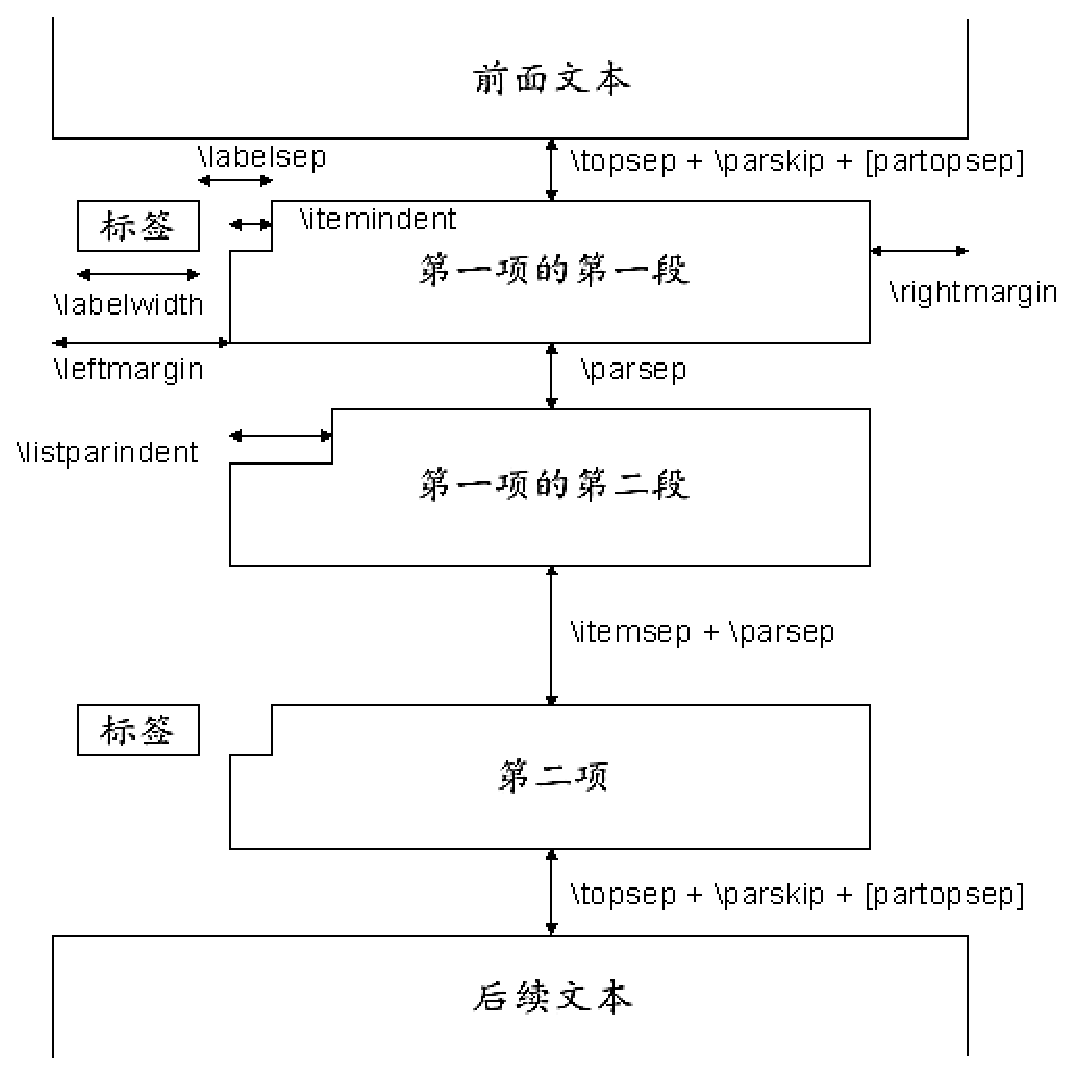
\includegraphics[width = 0.6\textwidth]{list}
\bicaption[list]{}{罗列环境参数示意图}{Fig.$\!$}{Schematic diagram of list environments}\vspace{-1em}
\end{figure}
通过调用~enumitem~宏包可以很方便地控制罗列环境的布局,其~format.tex~文件中的~\verb|\setitemize|~和~\verb|\setenumerate|~命令分别用来设置~\verb|itemize|~和~\verb|enumerate|~环境的样式参数。采用~\verb|itemize|~单层罗列环境的排版形式如下:
\begin{itemize}
\item 第一个条目文本内容
\item 第二个条目文本内容
\item 第三个条目文本内容
\end{itemize}
其代码如下
\begin{verbatim}
\begin{itemize}
  \item 第一个条目文本内容
  \item 第二个条目文本内容
  ...
  \item 第三个条目文本内容
\end{itemize}
\end{verbatim}
采用~\verb|enumerate|~单层罗列环境的排版形式如下:
\begin{enumerate}
\item 第一个条目文本内容
\item 第二个条目文本内容
\item 第三个条目文本内容
\end{enumerate}
其代码如下
\begin{verbatim}
\begin{enumerate}
  \item 第一个条目文本内容
  \item 第二个条目文本内容
  ...
  \item 第三个条目文本内容
\end{enumerate}
\end{verbatim}

\BiSection{算法}{Algorithm}

这是一个算法的例子,来自~worldguy@lilacbbs。建议将算法放在~minipage~环境中,避免算法出现在页面版心之外。

\begin{algorithm}
\KwIn{training samples, {$(d_i, d_j)_q$; $\mathbf{q}_i, \mathbf{q}_j \in C$,
$q\in \mathbf{Q}$} }
\KwOut{parameter setting $\lambda^T$}%

\For{$t$=1 to $T$}
{   
    $\lambda^{t+1}_n = \lambda^t_n + \eta (f_n(q, c, d_i) - f_n(q, c, d_j))$
 }
\end{algorithm}

%\KwIn{training samples, {$(d_i, d_j)_q$; $\mathbf{q}_i, \mathbf{q}_j \in C$,
%$q\in \mathbf{Q}$} }
%\KwOut{parameter setting $\lambda^T$}%
%
%\For{$t$=1 to $T$}
%{   
%    $\lambda^{t+1}_n = \lambda^t_n + \eta (f_n(q, c, d_i) - f_n(q, c, d_j))$
% }
%\end{algorithm}

算法环境中右侧空白比较多,若想把右侧的空白框减小,可以采用~minipage~环境实现。把~algorithm~环境放到~minipage~环境里面,并且加上选项[H]禁止算法浮动,下面给出一个例子。需要说明的是,一般不需要进行这种处理。算法标题可有可无,若有中英文标题,请使用~\verb|\AlgoBiCaption{中文标题}{英文标题}|。下面给出两个有标题的例子。需要说明的是,算法的标题是自动换行,没有必要手动换行。

\begin{minipage}{0.8\textwidth}\centering
\begin{algorithm}[H]
 \AlgoBiCaption{这是一个简短的算法中文图题}{This is the English caption of the algorithm}
  \KwIn{training samples, {$(d_i, d_j)_q$; $\mathbf{q}_i, \mathbf{q}_j
      \in C$, $q\in \mathbf{Q}$} }
 \KwOut{parameter setting
    $\lambda^T$}
 \For{$t$=1 to $T$} { $\lambda^{t+1}_n = \lambda^t_n +
    \eta (f_n(q, c, d_i) - f_n(q, c, d_j))$ }
\end{algorithm}
\end{minipage}


\begin{minipage}{0.9\textwidth}\centering
\begin{algorithm}[H]
 \AlgoBiCaption{这是一个算法的比较长的中文图题,需要换行,这里采用自动换行,如果手动换行会造成算法目录中同样出现断行}{This is a long English caption of the algorithm, a new line  required, and this a new line}
  \KwIn{training samples, {$(d_i, d_j)_q$; $\mathbf{q}_i, \mathbf{q}_j
      \in C$, $q\in \mathbf{Q}$} }
 \KwOut{parameter setting
    $\lambda^T$}
 \For{$t$=1 to $T$} { $\lambda^{t+1}_n = \lambda^t_n +
    \eta (f_n(q, c, d_i) - f_n(q, c, d_j))$ }
\end{algorithm}
\end{minipage}

\BiSection{定理定义}{Theorem and definition}

若需要书写定理定义等内容,而且带有顺序编号,需要采用如下环境。除了~\verb|proof|~环境之外,其余~9~个环境都可以有一个可选参数作为附加标题。

\begin{center}\vspace{0.5em}\noindent\wuhao\begin{tabularx}{0.7\textwidth}{lX|lX}
定理 & \verb|theorem|~环境 & 定义 & \verb|definition|~环境 \\
例 & \verb|example|~环境 & 算法 & \verb|algo|~环境 \\
公理 & \verb|axiom|~环境 & 命题 & \verb|proposition|~环境 \\
引理 & \verb|lemma|~环境 & 推论 & \verb|corollary|~环境 \\
注解 & \verb|remark|~环境 & 证明 & \verb|proof|~环境 \\
\end{tabularx}\end{center}